\chapter{System zarządzania wykrywanymi zachowaniami}
System zarządzania wykrywanymi zachowaniami stanowi główny element 
zarządzający danymi w projekcie. Komponent ten został zaimplementowany w języku \texttt{Java} z 
wykorzystaniem szkieletu aplikacji \texttt{Spring Boot}, co pozwoliło na uzyskanie wydajnego przetwarzania, 
skalowalności oraz modułowej architektury.

Głównym przeznaczeniem serwisu jest rola centralnego punktu integracyjnego całego systemu. 
Podsystem ten pośredniczy w komunikacji z modułami detekcji obrazu na żywo, 
przyjmując i weryfikując poprawność rejestrowanych incydentów, jak również udostępnia 
punkty końcowe wykorzystywane przez interfejs użytkownika. Serwis odpowiada za 
zarządzanie przechowywanymi danymi detekcji oraz udostępniania materiały wideo pełnych 
sekwencji detekcji do odczytu dla operatorów.

\section{Architektura modułu}

\subsection{Model składowania danych}
W celu zagwarantowania optymalnej wydajności i uniknięcia opóźnień podczas 
zapisu dużych plików, w infrastrukturze projektowej zaimplementowano hybrydowy model 
składowania danych. Do składowania różnych rodzajów danych zostały wykorzystane:
\begin{itemize}
    \item \textbf{Relacyjna baza danych (\texttt{PostgreSQL})} --- Odpowiada za składowanie ustrukturyzowanych danych mapowań przechowywanych nagrań oraz szablonów detekcji. W bazie danych przechowywane są również przekazywane przy zapisie nagrań wykrytych w nich elementów, z odpowiednimi znacznikami czasowymi.
    \item \textbf{Lokalny system plików (Pamięć dyskowa)} --- Stanowi fizyczny magazyn dla zapisywanych nagrań. Dane na dysku kategoryzowane wewnątrz struktury katalogów, których nazwy odpowiadają dacie rejestracji, a poszczególne pliki wideo posiadają w nazwie precyzyjny znacznik czasu ich zapisu, co umożliwia administratorom i operatorom, ich ręczną lokalizację bezpośrednio z poziomu systemu operacyjnego, gdyby zaszła taka potrzeba.
\end{itemize}

\begin{figure}[H]
    \centering

    \begin{subfigure}{\textwidth}
        \centering
        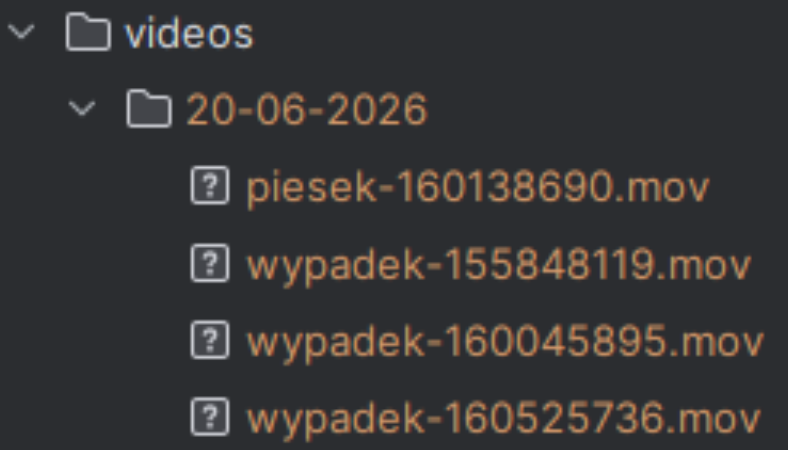
\includegraphics[width=0.4\linewidth]{images/przykladowy_stan_dysku_po_zapisie.png}
        \caption{Stan dysku z zapisanymi plikami nagrań detekcji.}
    \end{subfigure}

    \vspace{0.5cm}

    \begin{subfigure}{\textwidth}
        \centering
        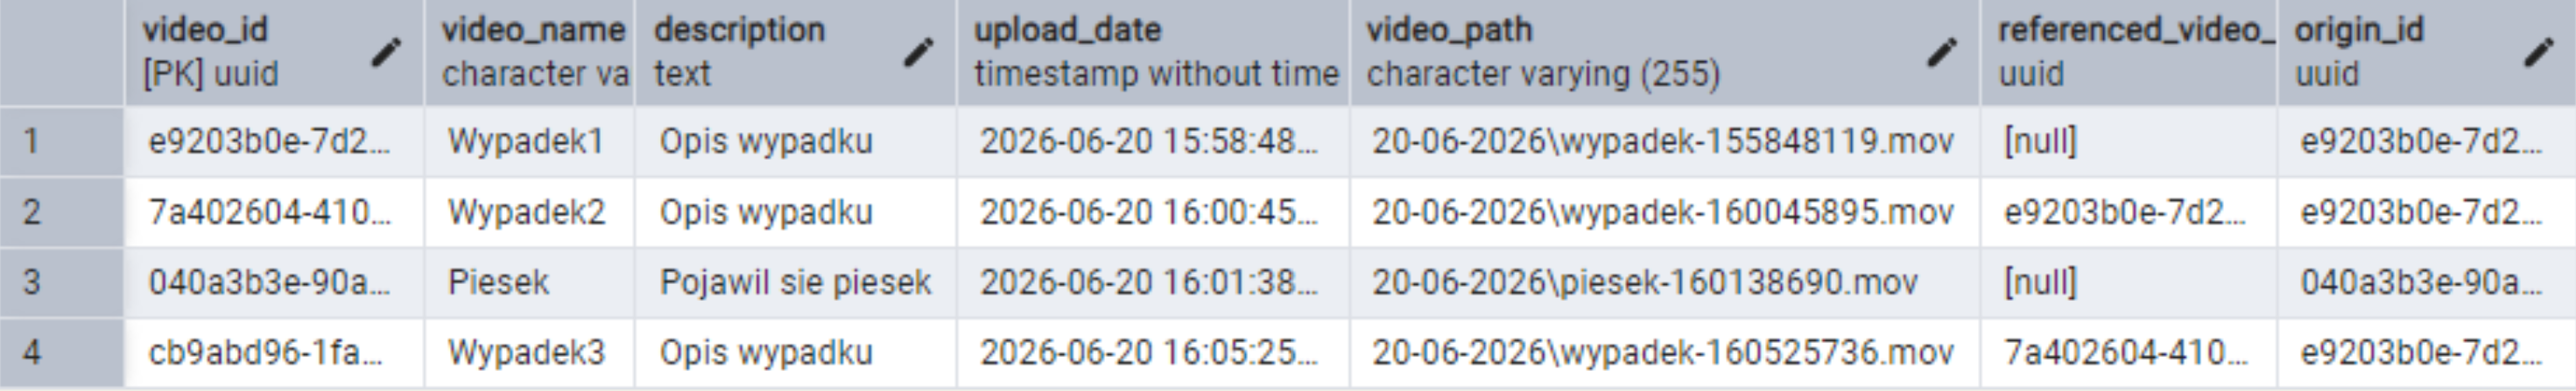
\includegraphics[width=0.95\linewidth]{images/przykladowy_stan_mapowan_w_bazie.png}
        \caption{Stan bazy danych ze zmapowanymi nagraniami.}
    \end{subfigure}

    \caption{Przykładowy stan dysku po zapisie nagrań fragmentów detekcji wraz z odzwierciedlającymi je mapowaniami zapisanymi w bazie danych.}
\end{figure}


\subsection{Architektura potoku zapisu i mapowania danych}
System zarządzania wykrywanymi zachowaniami w ramach zapisu i odczytu działa według zdefiniowanego potoku. 
Po wyemitowaniu przez detektor zestawu danych detekcji (pliku wideo wraz z opisem jego detekcji w formacie \texttt{JSON}), 
uruchamiana jest weryfikacja danych wejściowych. W ramach tej weryfikacji najpierw sprawdzana 
jest poprawność formatu pliku multimedialnego, co zapobiega próbom przesłania plików uszkodzonych 
lub obrazów statycznych zamiast strumienia wideo. Następnie system sprawdza poprawność składniową 
i budowę powiązanego dokumentu \texttt{JSON} zawierającego szczegóły detekcji.

Gdy walidacja zakończy się sukcesem, plik wideo jest fizycznie zapisywany w odpowiednim 
katalogu na dysku twardym. Po otrzymaniu systemowego potwierdzenia o prawidłowym zapisie pliku 
serwis zapisuje w bazie danych wiersz mapujący zapisany plik wideo w bazie \texttt{PostgreSQL}.
Rekord ten zawiera unikalne ID, ścieżkę dyskową oraz dwa kluczowe wskaźniki: 
\texttt{referenced\_video\_id} (ID filmu poprzedzającego w sekwencji) oraz 
\texttt{origin\_id} (ID elementu rozpoczynająca daną sekwencję wideo), co kończy proces zapisu.

Dopełnieniem potoku jest serwis synchronizujący, którego celem jest utrzymanie bezwzględnej 
spójności mapowań pomiędzy warstwą bazodanową a fizyczną zawartością dysku lokalnego. 
Ponieważ potok zapisu działa wieloetapowo, jakiekolwiek zakłócenia zewnętrzne 
(np.\ ręczne usunięcie pliku przez administratora lub awaria zasilania w trakcie trwania procedury) 
mogłyby doprowadzić do powstania mapowań wskazujących na nieistniejące zasoby. 
Z tego powodu serwis synchronizujący stale monitoruje efekty potoku zapisu, reagując natychmiastowo 
na zmiany w stanie plików, również w trakcie pracy systemu, Informując o dokonanych operacjach związanych
z synchronizacją. Zapewnia to, że przechowywane w bazie wiersze mapujące nagrania 
są zawsze bezwzględnym odzwierciedleniem stanu faktycznego zapisanych na dysku nagrań.

\begin{figure}[H]
    \centering
    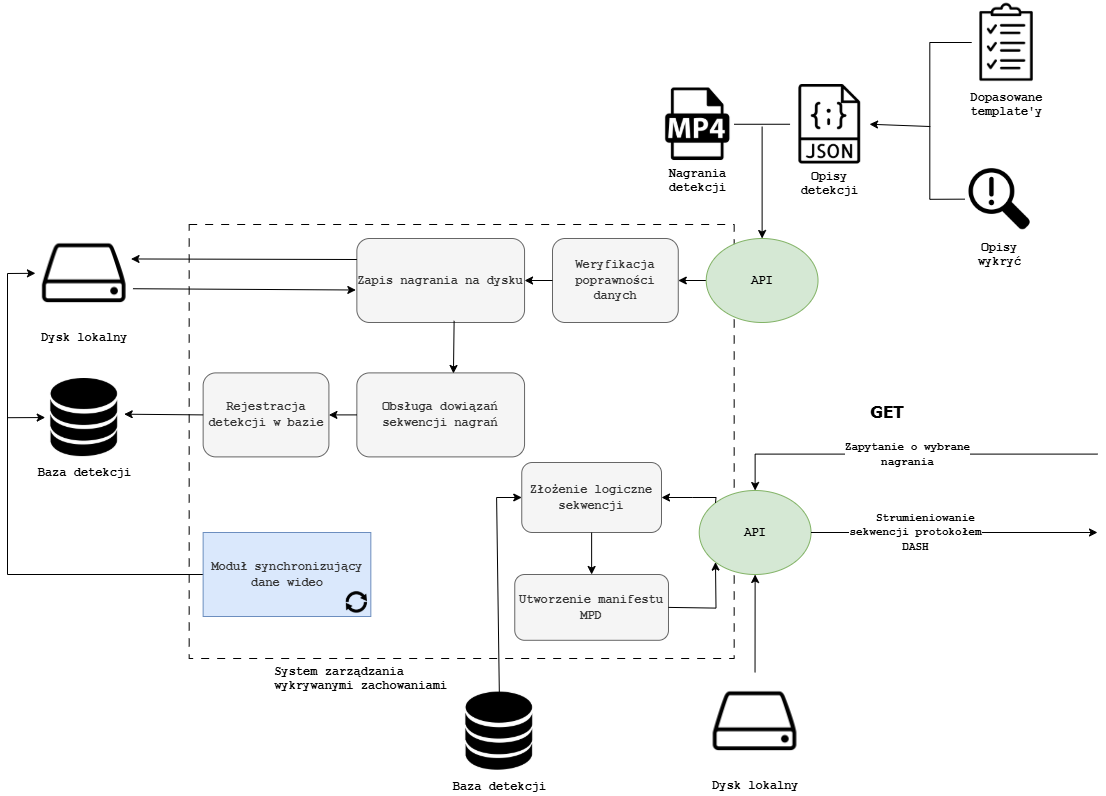
\includegraphics[width=0.9\textwidth]{images/diagram_backed.png}
    \caption{Architektura potoku zapisywania oraz odczytu i strumieniowania nagrań wideo.}
\end{figure}


\section{Opis funkcjonalności}

\subsection{Logika sekwencjonowania nagrań wideo}
Kluczową, w kontekście zapisywania nagrań z kamer, funkcjonalnością systemu jest możliwość 
rejestrowania długotrwałych zdarzeń bez przeciążania infrastruktury sieciowej. 
Funkcja ta realizowana jest poprzez mechanizm sekwencji, czyli logicznych list powiązanych, następujących
po sobie fragmentów wideo. Zamiast oczekiwać na zakończenie całego (możliwie kilkuminutowego) 
zdarzenia i wysyłać jeden duży plik, moduł detekcji sukcesywnie przesyła parosekundowe fragmenty detekcji. 
Zapewnia to informowanie operatorów o zagrożeniach w czasie rzeczywistym, co jest bardzo ważnym elementem, 
jeżeli system miałby zostać zastosowany w kontroli bezpieczeństwa.

Logika powiązań między nagraniami opiera się na strukturze listy jednokierunkowej 
generowanej w ramach zapisywanych mapowań do bazy danych. Jako ważne elementy sekwencji należy wymienić:
\begin{itemize}
    \item \textbf{origin} --- Pierwszy fragment rejestrujący początek incydentu. Wszystkie fragmenty należące do tego samego zdarzenia współdzielą ten sam \texttt{origin\_id}.
    \item \textbf{referenced\_video\_id} --- Każdy kolejny fragment przechowuje identyfikator swojego bezpośredniego poprzednika. Ten element bezpośrednio odpowiada za strukturę listy jednokierunkowej.
    %\item 
\end{itemize}
Zastosowanie wspólnego \texttt{origin\_id} eliminuje konieczność iteracyjnego, kosztownego przeszukiwania bazy „element po elemencie” podczas odczytu, kierując się jedynie dowiązaniami z \texttt{referenced\_video\_id}, przy wyszukiwaniu sekwencji. Zamiast tego system jednym zapytaniem \texttt{SQL} pobiera wszystkie rekordy o danym \texttt{origin\_id}, a dopiero następnie w pamięci \texttt{RAM} układane są one w prawidłowej kolejności przy wykorzystaniu \texttt{referenced\_video\_id}, przygotowując do wyświetlenia.

\begin{figure}[H]
    \centering
    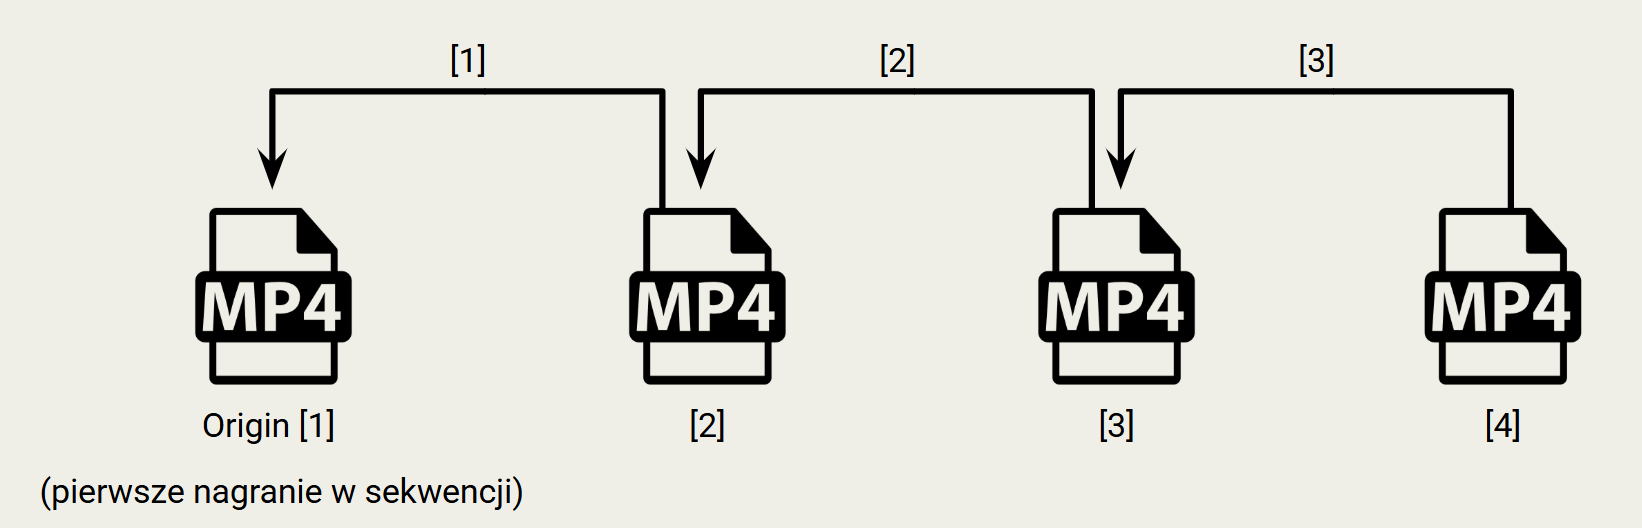
\includegraphics[width=0.8\textwidth]{images/przykladowa_sekwencja.png}
    \caption{Diagram logiczny struktury przykładowej sekwencji nagrań wideo.}
\end{figure}

\subsection{Mechanizm naprawy powiązań sekwencji}
System, poza usuwaniem całych sekwencji, pozwala z poziomu \texttt{API} na kasowanie pojedynczych, 
wybranych fragmentów z sekwencji danego zdarzenia. Rodzi to jednak ryzyko przerwania spójności 
referencyjnej i możliwości „osierocenia” pozostałych elementów sekwencji, co uniemożliwiłoby 
poprawne odtwarzanie filmu detekcji. W tym celu zaimplementowano mechanizm naprawy powiązań między 
elementami sekwencji. W jego ramach realizowane są trzy scenariusze:
\begin{enumerate}
    \item \textbf{Usunięty został element końcowy} --- Nie wymaga ingerencji, struktura listy pozostaje nienaruszona.
    \item \textbf{Usunięty został element środkowy} --- Algorytm modyfikuje mapowania fragmentów detekcji w bazie danych tak, aby element następujący po usuniętym wskazywał jako swój \texttt{referenced\_video\_id} na element stojący przed usuniętym fragmentem (przepięcie wskaźnika).
    \item \textbf{Usunięty został element inicjujący (origin)} --- Drugi w kolejności fragment w sekwencji zostaje pozbawiony wskaźnika \texttt{referenced\_video\_id} (staje się nowym początkiem, origin). We wszystkich elementach tej sekwencji wartość \texttt{origin\_id} zostaje nadpisana identyfikatorem nowego elementu początkowego.
\end{enumerate}

\subsection{Serwis synchronizujący mapowania danych}
Nad spójnością danych mapowań nagrań w bazie danych czuwa serwis synchronizujący. 
Zapobiega on powstawaniu martwych rekordów w bazie, gdy baza wskazuje na plik usunięty z poziomu dysku przez administratora. 
Usługa ta reaguje w trzech sytuacjach:
\begin{itemize}
    \item \textbf{Pomyślna weryfikacja startowa} --- Podczas uruchamiania serwisu system sprawdza zgodność mapowań w bazie z dyskiem. W przypadku pełnej spójności wysyłany jest komunikat potwierdzający integralność danych.
    \item \textbf{Synchronizacja przy rozruchu} --- Jeśli pliki zostały skasowane z dysku w czasie, gdy serwer był wyłączony, przy starcie system zidentyfikuje te braki i usuwa nieaktualne wpisy z bazy danych. Na koniec wyświetlany jest raport statystyczny informujący o liczbie usuniętych w ten sposób mapowań.
    \item \textbf{Synchronizacja w trakcie pracy systemu} --- Wszystkie modyfikacje plików na dysku podczas działania aplikacji są przechwytywane, a powiązane mapowania fragmentów nagrań w bazie, są również natychmiast usuwane.
\end{itemize}

\subsection{Zarządzanie szablonami detekcji}
Podsystem udostępnia pełną funkcjonalność zarządzania szablonami reguł za pośrednictwem \texttt{API} 
i powiązanego interfejsu webowego operatora. Użytkownik ma możliwość tworzenia, edycji, pobierania 
oraz usuwania konfiguracji szablonów. Każdy szablon ma unikalną nazwę oraz tablicę 
tzw.\ wektorów detekcji. Wektory definiują kombinacje oraz progi liczbowe obiektów 
(np.\ obecność minimum dwóch ludzi i jednego niebezpiecznego narzędzia). 
System udostępnia także dynamiczną listę aktualnie obsługiwanych klas obiektów, co pozwala 
interfejsowi webowemu na walidację wprowadzanych przez użytkownika definicji i zapobieganiu 
zapisywaniu błędnych reguł.

\subsection{Rejestracja i zapis nagrań detekcji}
Zapis fragmentów wideo oraz powiązanych z nimi opisów wykrytych elementów, otrzymanych 
bezpośrednio z modułu detektora, odbywa się za pośrednictwem punktu końcowego \texttt{REST API}.\
Ze względu na konieczność jednoczesnego przesyłania binarnego pliku multimedialnego (wideo) 
oraz ustrukturyzowanych danych tekstowych, żądanie to jest realizowane w formacie 
\texttt{multipart/form-data}. Format ten pozwala na niezależne przekazywanie różnych typów 
danych w ramach jednego zapytania \texttt{HTTP}.\

Po odebraniu tak sformułowanego żądania, system zarządzania wykrywanymi zachowaniami 
weryfikuje poprawność danych wejściowych, sprawdzając poprawność formatu pliku wideo, 
co zapobiega próbom przesłania plików uszkodzonych lub obrazów statycznych, 
a następnie waliduje budowę powiązanego dokumentu \texttt{JSON} zawierającego opis detekcji. 
Następnie plik wideo jest fizycznie zapisywany na dysku twardym w katalogu odpowiadającym dacie rejestracji, 
a do jego nazwy dopisywany jest precyzyjny znacznik czasowy. Dopiero po otrzymaniu potwierdzenia 
o prawidłowym zapisie pliku na dysku, serwis zapisuje w bazie \texttt{PostgreSQL} wiersz mapujący. 
Rekord ten wiąże fizyczny plik z unikalnym ID, ścieżką dostępu oraz wskaźnikami strukturalnymi 
sekwencji (\texttt{referenced\_video\_id} oraz \texttt{origin\_id}), co kończy proces zapisu.

W strukturze przesyłanego zapytania z modułu detekcji zawarte są następujące parametry wejściowe:
\begin{itemize}
    \item \texttt{file} --- Parametr zwierający surowe nagranie wideo z zarejestrowanym incydentem detekcji. Akceptowane są pliki w formacie \texttt{MP4} oraz \texttt{MOV}. Plik ten po przejściu walidacji formatu jest zapisywany w strukturze dyskowej serwera.
    \item \texttt{video-name}, \texttt{description} --- Określające nazwę oraz opis przypisane do danego fragmentu wideo. Wartości te nie są wykorzystywane w mapowaniu nagrania, a służą jedynie do wyświetlenia w interfejsie graficznym operatorowi.
    \item \texttt{relative-path} --- Ścieżka relatywna, która instruuje serwis, w jakim konkretnie miejscu wewnątrz katalogu nadrzędnego o określonej dacie ma zostać zapisany plik wideo na dysku lokalnym. Umożliwia to elastyczny zapis wideo mimo zastosowania automatycznie datowanych katalogów.
    \item \texttt{continuation-of} --- Opcjonalny parametr przechowujący identyfikator (ID) nagrania bezpośrednio poprzedzającego przesyłany fragment w strukturze sekwencji. Przekazanie tego parametru skutkuje automatycznym włączeniem nowego pliku do istniejącej już sekwencji wideo (jako kolejny element listy jednokierunkowej). W przypadku braku tego parametru system traktuje żądanie jako otwarcie zupełnie nowego incydentu i nadaje mu status elementu \textit{origin}.
    \item \texttt{details} --- Blok w formacie \texttt{JSON}, generowany moduł detektora. Zawiera on ustrukturyzowany opis detekcji, w tym wykaz klas wszystkich wykrytych obiektów oraz znaczniki czasowe określające zakres wykrycia elementów wewnątrz przesyłanego wideo.
\end{itemize}

\begin{figure}[H]
    \centering
    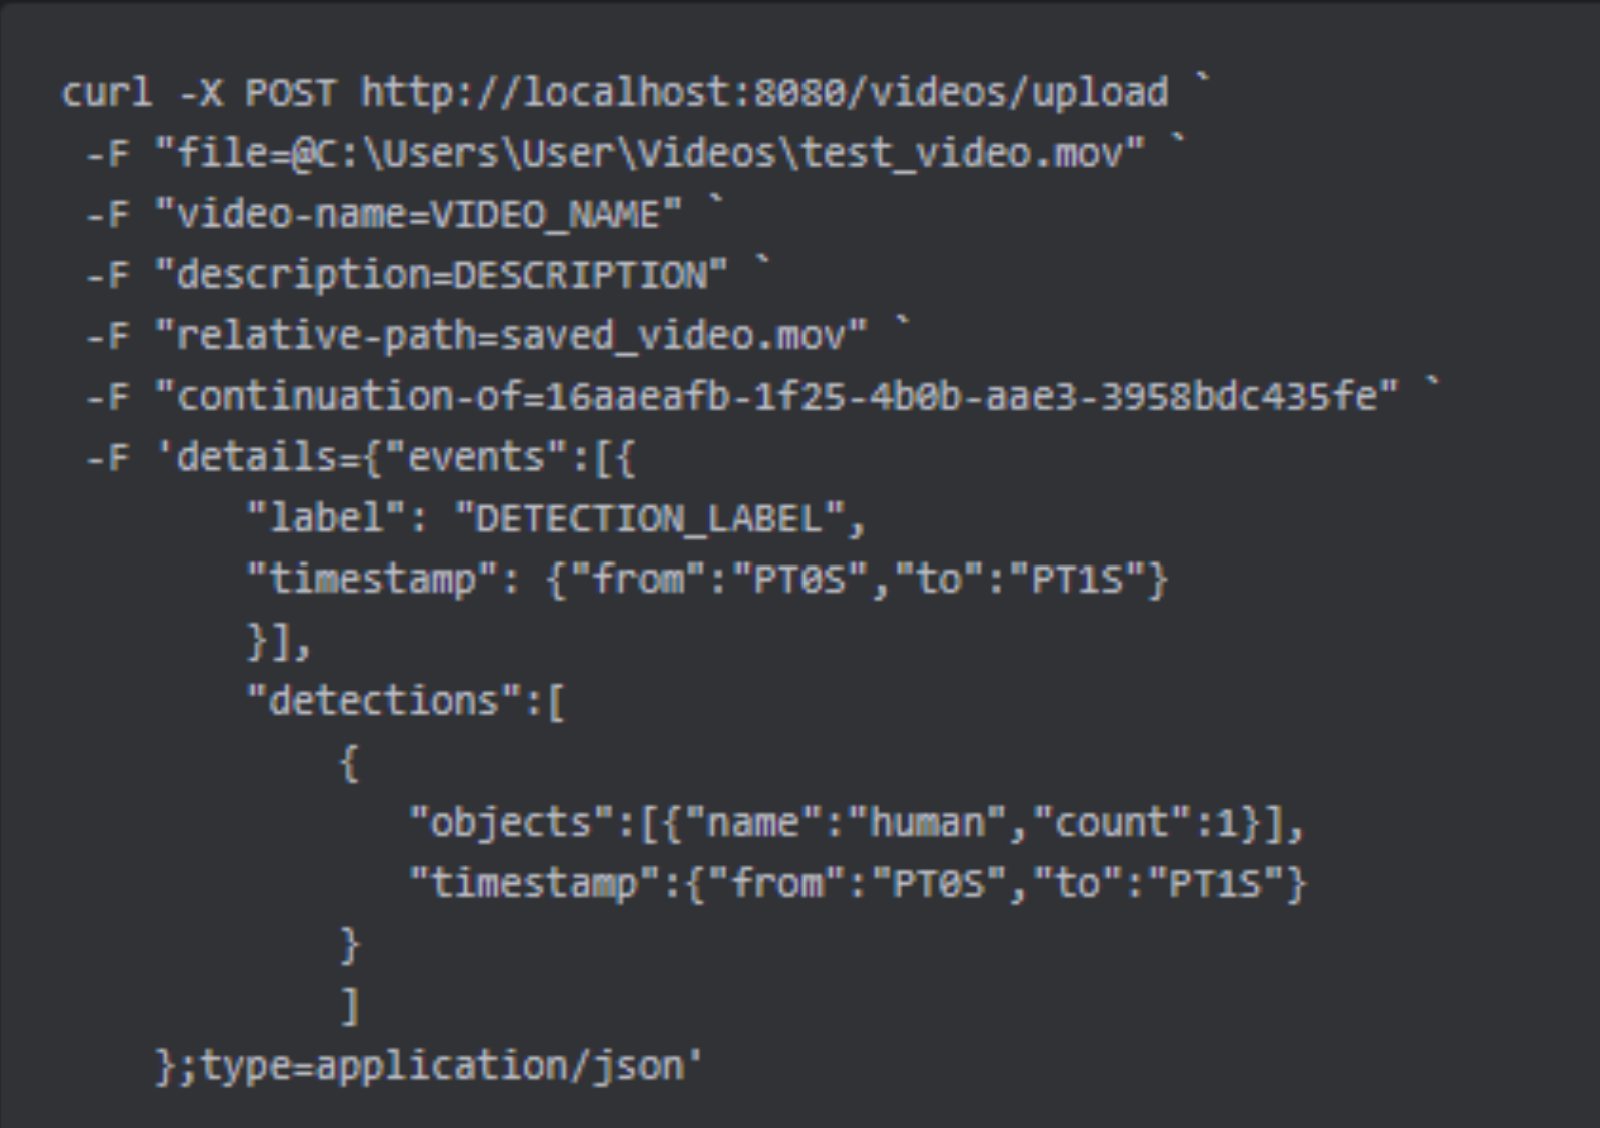
\includegraphics[width=0.8\textwidth]{images/przykladowe_zapytanie_zapisu_do_backendu.png}
    \caption{Przykładowe zapytanie zapisu detekcji.}
\end{figure}

\subsection{Strumieniowanie multimediów przy użyciu protokołu \texttt{DASH}}
Ostatnią kluczową funkcjonalnością jest dostarczanie wideo do interfejsu użytkownika obsługujące 
podzielone na fragmenty nagrania detekcji. System wykorzystuje do tego standard \texttt{DASH} 
(\textit{Dynamic Adaptive Streaming over HTTP}), opierając przesył danych o mechanizm częściowej 
zawartości (\textit{Partial Content}) przy wykorzystaniu kodu odpowiedzi \texttt{HTTP 206}. 

Na bazie logicznie ułożonej sekwencji, serwis generuje w locie manifest \texttt{XML} z rozszerzeniem 
\texttt{.mpd} (\textit{Media Presentation Description}). Dokument ten informuje odtwarzacz 
przeglądarki o osadzeniu czasowym poszczególnych fragmentów oraz adresach \texttt{URL}, 
pod którymi można je pobrać. Przeglądarka sekwencyjnie pobiera wyłącznie te fragmenty, 
które są niezbędne do zapełnienia bieżącego bufora odtwarzacza. 
Dla operatora korzystającego z interfejsu proces ten jest całkowicie niewidoczny. Pomimo 
fizycznego podzielenia danych na dysku, odtwarzany materiał zachowuje iluzję ciągłości nagrania,
przy jednoczesnym wyeliminowaniu opóźnień sieciowych i długiego buforowanie, jak w przypadku jednolitych
długich plików wideo.

\begin{figure}[H]
    \centering
    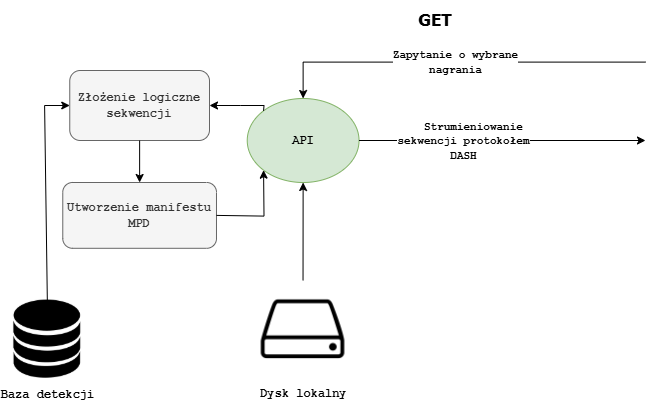
\includegraphics[width=0.7\textwidth]{images/Diagram_DASH.png}
    \caption{Potok odczytu sekwencji nagrań.}
\end{figure}